\documentclass[t,aspectratio=169]{beamer}

\usepackage{bm}
\usepackage{soul}
\usepackage{tikz}
\usepackage{tikz-3dplot}
\usepackage{amsmath}
\usepackage{amsfonts}
\usepackage{amssymb}
%\usepackage{physics}
%\usepackage{graphicx}
\usepackage{multicol}
\usepackage{t1enc}
\usepackage[utf8]{inputenc}
\usepackage[magyar]{babel}
\usepackage{pgfplots}
\pgfplotsset{compat=1.18}


\usetikzlibrary{calc,3d,decorations.pathmorphing,decorations.pathreplacing,decorations.markings,snakes,arrows.meta,calc,patterns}
\tikzset{snake it/.style={decorate, decoration=snake}}
% \usetheme{Madrid}
% \usecolortheme{whale}

%\usepackage{hyperref}
\hypersetup{
    colorlinks=true,
    linkcolor=blue,
    filecolor=magenta,      
    urlcolor=cyan,
    pdftitle={(KTXFI1EBNF) Physics I. Lecture},
}

% ----------------------------------------------------------------------------------------------------------------------------------------

\title{\includegraphics[width=45pt]{oepecsetlogo.png}\\(KTXFI1EBNF) Physics I. Lecture}

\author{Dr.~Gábor FACSKÓ, PhD\\\tiny Assistant Professor / Senior Research Fellow\\\textit{facsko.gabor@uni-obuda.hu}}

\institute{\Tiny Óbuda University, Faculty of Electrical Engineering, 1084 Budapest, Tavaszmező u. 17.\\Wigner Research Centre for Physics, Department of Space Physics and Space Technology, 1121 Budapest, Konkoly-Thege~Miklós~út~29–33.\\ \url{https://wigner.hu/~facsko.gabor}}

\date{April~20,~2026}

\logo{\includegraphics[height=0.9 true cm]{kekcsik.png}}

% ----------------------------------------------------------------------------------------------------------------------------------------

\begin{document}

\frame{\titlepage}

% ----------------------------------------------------------------------------------------------------------------------------------------

\begin{frame}
\frametitle{Current Updates and Announcements}
\begin{itemize}
\setlength{\parskip}{0pt}
\setlength{\itemsep}{4pt}
\item April 20, April 27, May 4, and go\dots
\item There will be one occasion without a lecture.
\item Homework No.~2 is now available soon. The deadline is May 4, 2026 at midnight.
\item Slides on Moodle: better oriented lecture, and practice with solution.
%\item Breaking News: I got full access to OpenAI for a month.
\end{itemize}
\end{frame}

% ----------------------------------------------------------------------------------------------------------------------------------------

%\begin{frame}[fragile,squeeze,allowframebreaks]
%  \frametitle{ChatGPT rulez}

%\begin{center}
%\includegraphics[yskip=-20pt,width=0.65\textwidth]{images-20260420/sith_facsko-20260417.png}
%\end{center}

%\pagebreak  
%\begin{center}
%\includegraphics[width=0.7\textwidth]{images-20260420/anatar_facsko-20260418.png}
%\end{center}

%\end{frame}

% ----------------------------------------------------------------------------------------------------------------------------------------

\begin{frame}[fragile,squeeze,allowframebreaks]
\frametitle{Where are we?}
\begin{enumerate}
\setlength{\parskip}{0pt}
\setlength{\itemsep}{0pt}
\item \textbf{Mechanics I.:} Newton’s laws, equation of motion (review). Momentum. General concept of mechanical work, work theorem. Forms of mechanical energy.
\item \textbf{Mechanics II.:} Weight force, gravitational force, gravitational field. Work of the gravitational force. Conservative force field. Dissipative force field. Mechanical power.
\item \textbf{Mechanics of Rigid Bodies I.} Concept of a rigid body. Forces acting on a rigid body. Motion of a rigid body. Concept of the centre of mass. Location of the centre of mass. Torque. Angular momentum. Energy of a rotating rigid body, angular momentum of a rotating rigid body, Steiner’s theorem.
\item \textbf{Mechanics of Rigid Bodies II.} Principal theorems of rigid body motion; conservation laws. Collisions.
\item \textbf{Oscillations I.} Dynamic condition of harmonic oscillatory motion. Differential equation of harmonic undamped oscillatory motion.
\pagebreak
\item \textbf{Oscillations II.} Superposition of oscillations. Decomposition of oscillations into components. Damped oscillations. Forced oscillations, resonance. Coupled oscillations.
\item \textbf{Wave phenomena:} Reflection of waves, refraction of waves, diffraction of waves. Huygens–Fresnel principle. Interference of waves. Polarization of waves.
\item \textbf{Elements of acoustics:} Basics of acoustics. Fundamental concepts. Doppler effect. Sound intensity, loudness according to Weber–Fechner’s law.
\item \textbf{Thermodynamics I:} Temperature scales, thermal expansion, thermometers. State variables, ideal gas, state changes, ideal gas equation of state, Boyle’s law, Gay-Lussac’s laws, universal (combined) gas law, heat, specific heat, molar heat, heat capacity.
\item \textbf{Thermodynamics II:} Expansion work, internal energy, the first law of thermodynamics, forms of the first law in different state changes.
\pagebreak
\vskip -10 pt
\item \textbf{Thermodynamics III:} Cyclic processes, Carnot cycle, Carnot’s theorem, reduced heat, entropy, the second law of thermodynamics.
\item \textbf{Thermodynamics IV:} Kinetic theory of gases, molecular thermodynamics. Distributions, distribution functions. Elementary statistics.
\item \textbf{Electrostatics I.:} Electric charge: Fundamental electrical phenomena, electric charge and matter, Coulomb’s law (force between two point charges, unit of electric charge, permittivity of vacuum).
\item \textbf{Electrostatics II.:} The electric field: The electrostatic field (electric field strength, electric field lines). Determination of electric field strength. Gauss’s law (flux of the electric field). Electric field of a point charge.
\pagebreak
\item \textbf{Electrostatics III.:} \textit{Electrostatic potential: Work of the electric field (work done in an electric field). Electric potential (electrostatic potential). Electric potential difference, voltage. Electric potential of charge systems at small and large distances. Electrostatic energy.}
\item \textbf{Elements of physical or wave optics.} Branches of optics. Light interference, light diffraction, diffraction through a slit, optical grating, light polarization. Light as an electromagnetic wave: Poynting vector. Optical instruments.
\end{enumerate}
\end{frame}

% ----------------------------------------------------------------------------------------------------------------------------------------

% Slide 1: Fundamental Electrical Phenomena
\begin{frame}[fragile,squeeze,allowframebreaks]
\frametitle{Electrostatic Potential}
\begin{itemize}
\setlength{\parskip}{0pt}
\setlength{\itemsep}{4pt}
\item \textbf{Work Done in an Electric Field}
\vskip -15 pt
\begin{columns}
  \begin{column}{0.4\linewidth}
    \vfill
\begin{center}
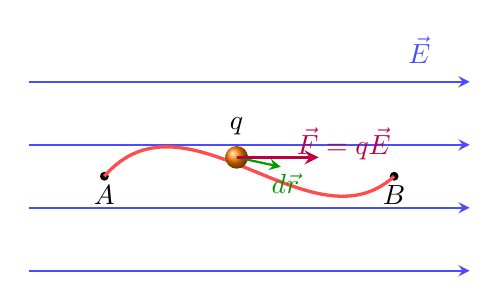
\begin{tikzpicture}[scale=0.8, >=stealth]

% Electric field lines
\foreach \y in {0.5,1.5,2.5,3.5} {
    \draw[->, thick, blue!70] (0,\y) -- (7,\y);
}

% Label for electric field
\node[blue!70] at (6.2,4.0) {$\vec{E}$};

% Points A and B
\fill (1.2,2) circle (2pt);
\node[below] at (1.2,2) {$A$};

\fill (5.8,2) circle (2pt);
\node[below] at (5.8,2) {$B$};

% Curved path from A to B
\draw[very thick, red!70] 
    (1.2,2) .. controls (2.5,3.5) and (4.5,0.8) .. (5.8,2);

% Charge q (on the path)
\shade[ball color=orange] (3.3,2.3) circle (0.18);
\node[above] at (3.3,2.5) {$q$};

% Small tangent segment (dr)
\draw[->, thick, green!60!black] 
    (3.3,2.3) -- (4.0,2.15);
\node[below right,green!60!black] at (3.7,2.2) {$d\vec{r}$};

% Force vector (same direction as E)
\draw[->, very thick, purple] 
    (3.3,2.3) -- (4.6,2.3);
\node[above right, purple] at (4.1,2.1) {$\vec{F}=q\vec{E}$};

% Caption formula
%\node[align=center] at (3.5,0.2) {$\displaystyle
%W_{A\to B}=\int_A^B \vec{F}\cdot d\vec{r}
%= q\int_A^B \vec{E}\cdot d\vec{r}$};

\end{tikzpicture}
\end{center}
\end{column}
\begin{column}{0.6\linewidth}

\item When a charge $q$ moves in an electric field $\vec{E}$, the electric force is
$$ \vec{F} = q\vec{E}. $$

\item The work done by the electric field when the charge moves from point $A$ to point $B$ is
$$ W_{A \to B} = \int_A^B \vec{F}\cdot d\vec{r} = q\int_A^B \vec{E}\cdot d\vec{r}.$$


\end{column}
\end{columns}
\item The work depends on the electric field and the path.
\item In electrostatics, the field is conservative.
\item Therefore, the work depends only on the initial and final points.

\pagebreak
\item \textbf{Conservative Nature of the Electrostatic Field:} For an electrostatic field,
$$ \oint \vec{E}\cdot d\vec{r} = 0.$$

\item Therefore,
\begin{itemize}
\item The total work along any closed path is zero.
\item We can define a scalar quantity called \textbf{electric potential}.
\item It is often easier to work with potential than with force.
$$ W_{A \to B} = -\Delta U = -(U_B-U_A), $$ where $U$ is the electric potential energy.
\end{itemize}

\item \textbf{Remember: Gravity!!!}

\pagebreak
\item \textbf{Electric Potential and Voltage:} The \textbf{electric potential} (electrostatic potential) is the potential energy per unit charge:
$$ V = \frac{U}{q}. $$
\item The potential difference between points $A$ and $B$ is
$$ V_B - V_A = -\int_A^B \vec{E}\cdot d\vec{r}. $$

\begin{itemize}
\item Unit of potential: volt (V)
\item $1\,\text{V} = 1\,\text{J/C}$
\item Potential is a scalar quantity
\end{itemize}

\pagebreak
\item \textbf{Potential Difference and Voltage:} The \textbf{voltage} between two points is their potential difference:
$$ U_{AB} = V_A - V_B. $$

\item Important comments:
\begin{itemize}
\item If a positive charge moves in the direction of the electric field, the potential decreases.
\item The electric field points from higher potential to lower potential.
\item Relation between field and potential:
$$\vec{E} = -\nabla V. $$
\end{itemize}

\item \textbf{Remark:} $\nabla = \left(\frac{\partial}{\partial x},\frac{\partial}{\partial y},\frac{\partial}{\partial z}\right)$, gradient, divergence, rotation. 


\pagebreak
\item \textbf{Potential of a Point Charge}
\vskip -15 pt
\begin{columns}
\begin{column}{0.4\linewidth}
\vfill
\begin{center}
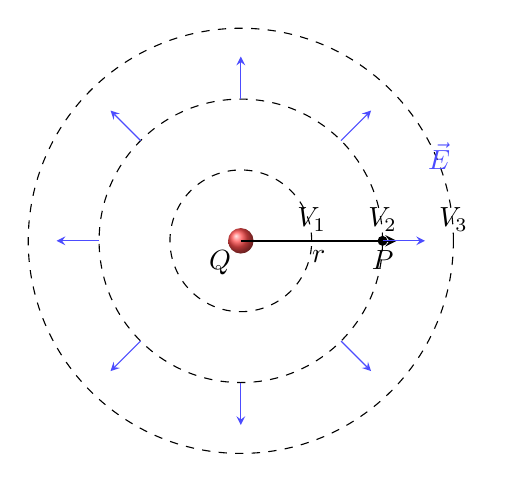
\begin{tikzpicture}[scale=0.9, >=stealth]

% Center charge
\shade[ball color=red!70] (0,0) circle (0.18);
\node[below left] at (0,0) {$Q$};

% Equipotential circles
\draw[dashed] (0,0) circle (1);
\draw[dashed] (0,0) circle (2);
\draw[dashed] (0,0) circle (3);

% Labels for potentials
\node at (1,0.3) {$V_1$};
\node at (2,0.3) {$V_2$};
\node at (3,0.3) {$V_3$};

% Radial line (distance r)
\draw[->, thick] (0,0) -- (2.2,0);
\node[below] at (1.1,0) {$r$};

% Observation point
\fill (2,0) circle (2pt);
\node[below] at (2,0) {$P$};

% Electric field arrows (radial)
\foreach \angle in {0,45,90,135,180,225,270,315} {
    \draw[->, blue!70] 
        ({2*cos(\angle)}, {2*sin(\angle)}) 
        -- ({2.6*cos(\angle)}, {2.6*sin(\angle)});
}

% Label for E field
\node[blue!70] at (2.8,1.2) {$\vec{E}$};

% Potential formula
%\node[align=center] at (0,-3.5) {$\displaystyle
%V(r)=\frac{1}{4\pi\varepsilon_0}\frac{Q}{r}
%$};
\end{tikzpicture}
\end{center}
\end{column}
\begin{column}{0.6\linewidth}  
\item For a point charge $Q$, the electric potential at distance $r$ is
\vskip -15 pt
$$V(r) = \frac{1}{4\pi\varepsilon_0}\frac{Q}{r},$$
\vskip -5 pt
if we choose $V(\infty)=0$.

\begin{itemize}
\item If $Q>0$, then $V>0$
\item If $Q<0$, then $V<0$
\item Potential decreases as $1/r$
\end{itemize}

\item The electric field of a point charge is
$$E(r) = \frac{1}{4\pi\varepsilon_0}\frac{|Q|}{r^2}.$$
\end{column}
\end{columns}

\pagebreak
\item \textbf{Potential of Several Charges:} For a system of point charges, potentials add algebraically:
$$ V(\vec{r}) = \sum_i \frac{1}{4\pi\varepsilon_0}\frac{q_i}{r_i}, $$
where $r_i$ is the distance from charge $q_i$ to the observation point.

\begin{itemize}
\item Potential obeys the superposition principle.
\item Since potential is a scalar, addition is simpler than for electric field.
\end{itemize}

\item For a continuous charge distribution:
$$ V(\vec{r}) = \frac{1}{4\pi\varepsilon_0}\int \frac{dq}{r}. $$

\pagebreak
\item \textbf{Potential at small distances:}
\begin{itemize}
\item The nearest charges have the strongest effect.
\item The detailed geometry of the charge system is important.
\end{itemize}

\item \textbf{Potential at large distances:}
\begin{itemize}
\item A finite charge system often behaves like a single effective charge.
\item If the total charge is $Q_{\text{tot}}$, then approximately
$$ V(r) \approx \frac{1}{4\pi\varepsilon_0}\frac{Q_{\text{tot}}}{r}. $$
\end{itemize}
\item If the total charge is zero, the leading term may be a dipole term, which decreases faster with distance.

\pagebreak
\item \textbf{Example: Electric Dipole:} An electric dipole consists of charges $+q$ and $-q$ separated by a small distance.
\begin{itemize}
\item Close to the dipole, the potential depends strongly on position.
\item Far from the dipole, the potential is much smaller than for a single charge.
\end{itemize}
\item For large distances, the dipole potential behaves approximately as
$$ V(r,\theta) \sim \frac{\cos\theta}{r^2}. $$
\item Therefore,
\begin{itemize}
\item point charge: $V \sim 1/r$
\item dipole: $V \sim 1/r^2$
\end{itemize}

\end{itemize}
\end{frame}

% ----------------------------------------------------------------------------------------------------------------------------------------

%\section{Electrostatic Energy}

\begin{frame}[fragile,squeeze,allowframebreaks]
\frametitle{Electrostatic Potential Energy}
\begin{itemize}
\setlength{\parskip}{0pt}
\setlength{\itemsep}{4pt}
\item If a charge $q$ is placed at a point where the potential is $V$, then its \textbf{potential energy} is
$$ U = qV.$$

\item For two point charges:
$$ U = \frac{1}{4\pi\varepsilon_0}\frac{q_1 q_2}{r}.$$ 
\item Interpretation:
\begin{itemize}
\item $U>0$: energy must be supplied to assemble the system
\item $U<0$: energy is released when the system is assembled
\end{itemize}

\pagebreak
\item \textbf{Electrostatic Energy of a Charge System:} For many point charges, the total electrostatic energy is
$$
U = \frac{1}{2}\sum_i q_i V(\vec{r}_i),
$$
where $V(\vec{r}_i)$ is the potential produced by all other charges at the position of $q_i$.

\item Equivalent form:
$$
U = \frac{1}{4\pi\varepsilon_0}\sum_{i<j}\frac{q_i q_j}{r_{ij}}.
$$

\begin{itemize}
\item The factor $\tfrac{1}{2}$ avoids double counting.
\item This energy is stored in the electric configuration.
\end{itemize}

\pagebreak
\item \textbf{Energy Stored in the Electric Field:} Electrostatic energy can also be described as energy stored in the field itself.

\item The energy density is
$$ u = \frac{1}{2}\varepsilon_0 E^2. $$

\item So the total energy is
$$ U = \int u\, d\tau = \frac{1}{2}\varepsilon_0 \int E^2\, d\tau. $$

\item This form is especially useful for continuous charge distributions and capacitors.

\end{itemize}
\end{frame}

% ----------------------------------------------------------------------------------------------------------------------------------------


\begin{frame}
%\frametitle{Minden jó, ha a vége jó}

\vfill
\begin{center}
\textbf{\huge The End}

\bigskip
Thank you for your attention!
\end{center}
\vfill
%\textbf{Acknowledgements} Thank you for the course materials for Szilárd~ZSÓKA and Zoltán~VARGA.
\end{frame}

\end{document}
